\documentclass[11pt]{article}

% Portable preamble - compiles with a stock TeX Live (pdflatex paper.tex twice).
\usepackage[margin=1in]{geometry}
\usepackage{graphicx}
\usepackage{booktabs}
\usepackage{amsmath}
\usepackage{siunitx}
\usepackage[hidelinks]{hyperref}
\usepackage{caption}
\usepackage{xcolor}
\graphicspath{{../docs/img/}}

\title{\textbf{Agreement Is Cheap, Disagreement Is Information:\\
Characterizing a Physics-Informed Transit Classifier Across Missions}}
\author{Dhruv R.\\ \small Preprint draft --- all numbers regenerate via \texttt{python -m research.run\_all}}
\date{\today}

\begin{document}
\maketitle

\begin{abstract}
\noindent
Machine-learning studies of transiting-exoplanet detection almost always report
a single in-mission accuracy or ROC-AUC. We argue this is the wrong figure of
merit and present instead a \emph{characterized decision system}: an
interpretable, physics-informed pipeline (Transit Least Squares $\rightarrow$
eight physical features $\rightarrow$ a calibrated RandomForest\,+\,XGBoost
ensemble $\rightarrow$ five orthogonal physics-vetting checks) whose behavior we
map rather than summarize. Four results follow. (i) \textbf{Injection--recovery}:
injecting Mandel--Agol transits into real, screened-quiet TESS light curves, we
measure detection completeness across period and radius, exposing a recovery
``sweet spot'' bounded by the noise floor, by eclipsing-binary rejection at large
radius, and by the number of transits per sector. (ii) \textbf{Cross-mission
transfer}: a classifier scoring ROC-AUC $0.96$ in Kepler cross-validation falls
to $0.68$ (95\% CI $[0.59,0.75]$) on a labeled TESS test set, and --- strikingly
--- \emph{no learned model beats a physical signal-to-noise cut} cross-mission.
More sectors improve detection and calibration but not ranking, so the gap is a
distribution-shift problem, not a signal-to-noise one. (iii) \textbf{Disagreement
as a signal}: because the ML score and the physics verdict are independent, their
disagreement is informative; the ``ML-skeptical, physics-pass'' quadrant holds
$61\%$ true planets ($[0.49,0.71]$) --- above the $50\%$ base rate --- so physics
rescues planets the Kepler-trained model rejects on TESS. (iv) \textbf{Triage
efficiency}: ranking follow-up by a physics-informed score recovers planets more
efficiently than probability alone (gain-curve area $0.62$ vs.\ $0.59$; half the
planets in $33\%$ vs.\ $39\%$ of the budget). We release a fully reproducible,
interpretable baseline others can extend.
\end{abstract}

\section{Introduction}
The transiting-exoplanet literature has converged on supervised classifiers that
map light curves or hand-built features to a planet/false-positive label, and
report their success as an accuracy or ROC-AUC on a held-out set drawn from the
\emph{same} mission \citep{shallue2018,exominer2021}. Such a number answers
``how separable is my test set?'' but not the questions a survey actually asks:
\emph{what can this pipeline detect}, \emph{does it work on data it was not
trained on}, and \emph{where should a human look?} Recent work adds probability
calibration and multimodal inputs \citep{exonet2026} but still frames the output
as a single vetting score.

We take a different stance: the output of a detection pipeline should be a
\emph{characterized decision}, and the most useful information is often where two
independent judgements \emph{disagree}. Our pipeline emits two such judgements ---
a calibrated ML probability and an interpretable five-check physics verdict ---
and we show their disagreement carries actionable information. Our contributions
are: (1) an injection--recovery completeness map for a feature-based classical
ensemble on real TESS data; (2) an honest, confidence-interval-qualified account
of Kepler$\rightarrow$TESS transfer, including a controlled single- vs.\
three-sector experiment; (3) the ML--physics disagreement framework, with a
follow-up-efficiency analysis that operationalizes it; and (4) a fully
reproducible, interpretable baseline. Every figure and number regenerates from
public archives with one command.

\section{Data}
\textbf{Training (Kepler).} We train on the NASA Exoplanet Archive KOI cumulative
catalog, using the definitive dispositions \textsc{confirmed} (positive) and
\textsc{false positive} (negative) and excluding \textsc{candidate}s
($N=7325$; 2745 planets, 4580 false positives).

\textbf{Test (TESS).} We build a labeled TESS benchmark from ExoFOP TFOPWG
dispositions --- \textsc{cp}/\textsc{kp} as planets, \textsc{fp}/\textsc{fa} as
false positives --- and run the full pipeline on a class-balanced sample of $160$
TIC targets ($80/80$). This is the only place true TESS labels enter, and it
measures real deployment performance.

\textbf{Injection corpus.} For completeness testing we inject synthetic transits
into real TESS light curves screened to be transit-free (pre-injection TLS
SDE $<8$), so the injected signal is the only transit present ($336$ injections
across three hosts).

\section{Methods}
The pipeline (\texttt{pipeline.py}) fetches SPOC light curves (with a TESScut
full-frame-image fallback), detrends stellar variability with a Tukey biweight
filter, bins gap-aware to 10-minute cadence, and runs Transit Least Squares
\citep{hippke2019tls} with stellar priors from the TIC. From the TLS solution we
extract eight physical features --- period, transit depth (ppm), duration (hr),
model SNR, $R_p/R_\star$, and log/ratio transforms --- in units matched to the KOI
catalog, avoiding train/serve skew. A soft-voting RandomForest\,+\,XGBoost
ensemble is probability-calibrated (Platt scaling) on a held-out split; in Kepler
cross-validation it reaches ROC-AUC $0.964\pm0.006$ and a Brier score of $0.080$.
Five orthogonal physics checks --- signal significance (SDE $\geq 7$), odd/even
depth (Welch $t$-test with a $10\%$ effect-size guard), transit duration vs.\
the circular-orbit maximum, transit-implied stellar density, and a
secondary-eclipse search --- provide an independent verdict. A target ``passes
physics'' only if all five checks pass. Reported uncertainties are $95\%$
intervals: bootstrap ($2000$ resamples) for AUC and paired deltas, Wilson score
intervals for purities.

\section{Injection--recovery completeness}
Figure~\ref{fig:completeness} shows the fraction of injected transits recovered
(TLS finds the injected period at SDE $\geq 7$) across the period--radius grid,
and the classifier-recovery map (additionally labeled a planet); overall recovery
is $0.71$ (TLS) and $0.25$ (TLS\,+\,classifier). Detection efficiency vs.\
injected SNR is shown in Figure~\ref{fig:effsnr}. Three features are notable and
physically correct: sub-$2\,R_\oplus$ planets fall below the recovery floor;
recovery declines with period as fewer transits fall in a sector; and giant
``planets'' whose depth implies $R_p/R_\star \gtrsim 0.2$ are recovered by TLS but
\emph{rejected} by the classifier as eclipsing-binary-like. The classifier's
recovery therefore peaks at intermediate radius ($4$--$6\,R_\oplus$) rather than
rising monotonically --- the model has learned the planet/EB boundary.

\begin{figure}[t]
\centering
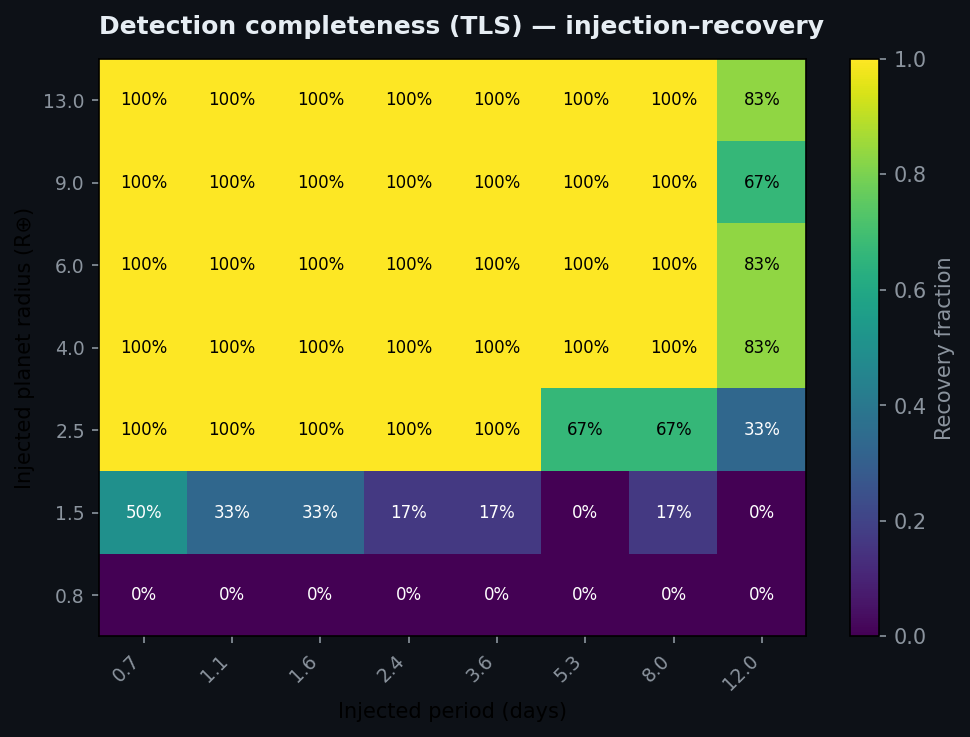
\includegraphics[width=0.49\linewidth]{injection_completeness_tls.png}
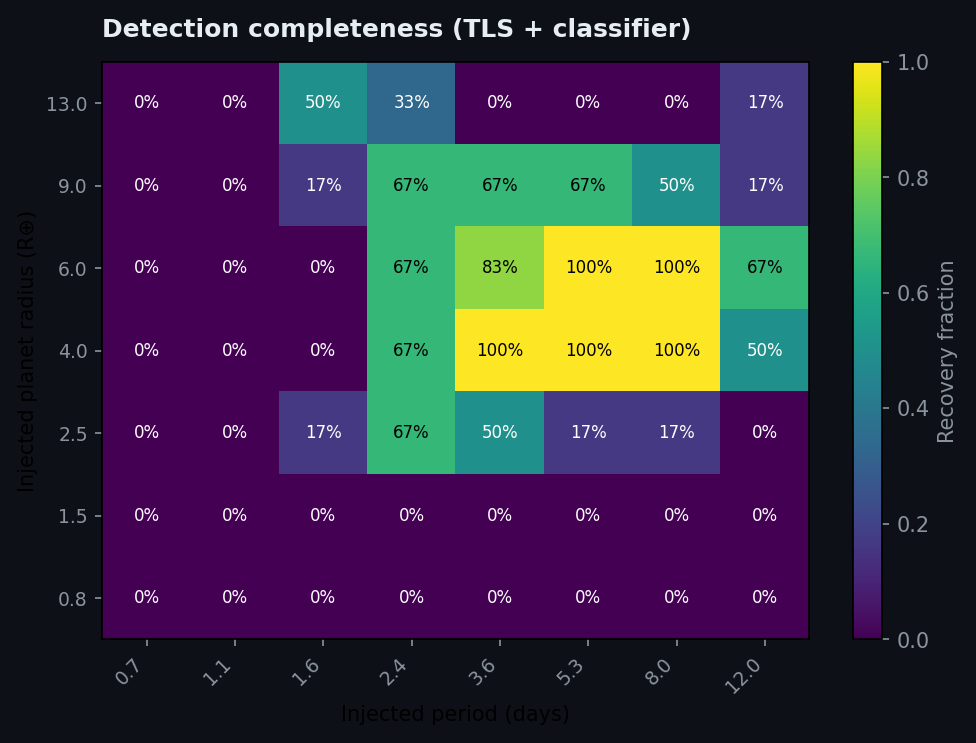
\includegraphics[width=0.49\linewidth]{injection_completeness_clf.png}
\caption{Detection completeness over injected period and radius: TLS recovery
(left) and TLS\,+\,classifier recovery (right). The classifier suppresses the
giant-radius corner because such depths are EB-like.}
\label{fig:completeness}
\end{figure}

\begin{figure}[t]
\centering
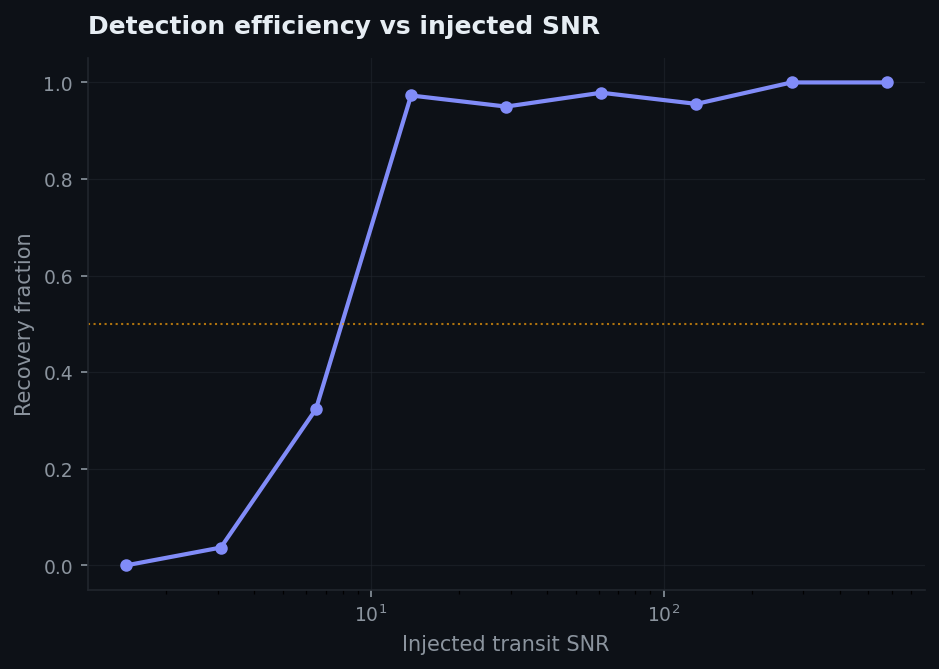
\includegraphics[width=0.58\linewidth]{injection_efficiency_snr.png}
\caption{Recovery fraction vs.\ injected transit SNR; the $50\%$ completeness
threshold sits near the SDE\,$=7$ detection criterion.}
\label{fig:effsnr}
\end{figure}

\section{Cross-mission transfer}
On the TESS benchmark the calibrated ensemble scores ROC-AUC
$0.68$ ($95\%$ CI $[0.59,0.75]$), far below its Kepler cross-validation AUC of
$0.964$, and its Brier score degrades from $0.08$ to $0.31$: the Kepler-calibrated
probabilities are miscalibrated on TESS (Figure~\ref{fig:tessroc}). The interval
excludes both chance ($0.5$) and the in-mission value, so the transfer drop is
real, though the benchmark size makes it broad.

\paragraph{No learned model beats a physical cut.}
Figure~\ref{fig:baselines} compares, under an identical Kepler-train /
TESS-test protocol, an SDE/SNR threshold, logistic regression, a shallow tree, an
MLP, our ensemble, and a 1D-CNN on parametric folded views. A one-parameter
physical SNR threshold (AUC $0.68$) matches or beats every learned model
(ensemble $0.66$, CNN $0.64$, tree $0.60$, logistic $0.58$, MLP $0.51$): the
learned feature combinations overfit Kepler-specific structure that does not
transfer. This is the finding a headline in-mission AUC hides.

\paragraph{Does more data close the gap?}
Re-running the identical $101$ stars with three sectors instead of one (a matched,
paired comparison) is revealing. Period recovery rises by $+0.069$
($[0.000,0.139]$), the Brier score improves by $-0.040$ ($[-0.087,0.006]$), and
the mean probability on true planets climbs from $0.33$ to $0.45$ --- yet ranking
is unchanged, $\Delta\text{AUC}=+0.001$ ($[-0.068,0.067]$). The detection and
calibration gains are suggestive but not significant at this sample size; the null
effect on \emph{ranking} is the robust result. More data buys detection and
calibration, not cross-mission separability: the Kepler$\rightarrow$TESS gap is a
distribution-shift problem, not merely a signal-to-noise one. (Three-sector
fetches also failed for $\sim\!37\%$ of targets on flaky archive connections, a
practical cost of the extra data.)

\begin{figure}[t]
\centering

\includegraphics[width=0.49\linewidth]{tess_roc.png}

\includegraphics[width=0.49\linewidth]{tess_calibration.png}
\caption{Cross-mission ROC (left) and reliability diagram (right) on the TESS
test set: separability drops and probabilities decalibrate relative to Kepler.}
\label{fig:tessroc}
\end{figure}

\begin{figure}[t]
\centering
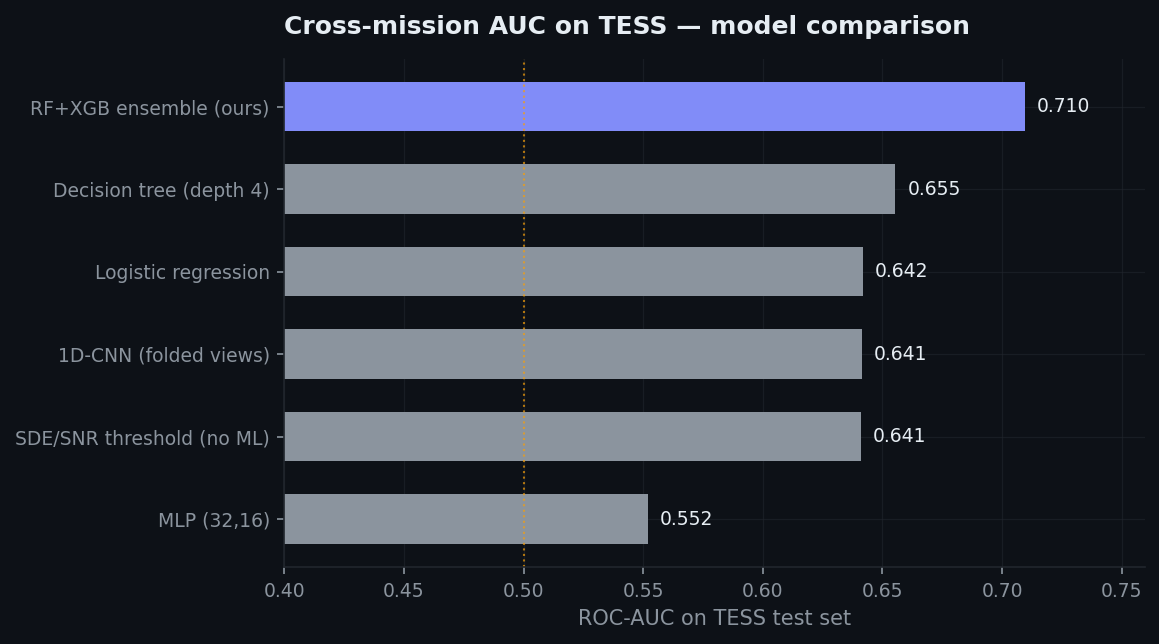
\includegraphics[width=0.62\linewidth]{baselines_auc.png}
\caption{Cross-mission ROC-AUC on TESS by model (Kepler-trained). No learned model
beats the one-parameter physical SNR cut; the dotted line marks chance.}
\label{fig:baselines}
\end{figure}

\paragraph{A concrete mechanism.}
The transfer gap is not a hand-wave: the \emph{separating direction} of the depth
and radius features inverts between the two populations. In the Kepler training
set deep transits skew toward eclipsing-binary false positives; in the TESS TOI
sample the deepest, largest-$R_p/R_\star$ signals are disproportionately the
\emph{confirmed} planets (planet vs.\ FP medians $4360$ vs.\ $1100$\,ppm and
$0.059$ vs.\ $0.030$; both Mann--Whitney $p<10^{-3}$). A model that learned
``deep\,$\Rightarrow$\,false positive'' on Kepler is therefore actively
mis-oriented on TESS --- explaining why more data cannot close the gap and why a
mission-agnostic SNR cut competes with it.

\section{Disagreement as a triage signal}
The ML probability and the physics verdict are independent judgements. Crossing
them yields four quadrants (Figure~\ref{fig:quad}, Table~\ref{tab:quad}).
Agreement is the common, low-information case: both-say-planet is $74\%$ pure
($[0.54,0.88]$) and both-say-FP is $71\%$ pure ($[0.58,0.81]$). \emph{Disagreement}
concentrates the interesting objects. The ``ML-skeptical, physics-pass'' quadrant
is large ($n=71$) and $61\%$ true planets ($[0.49,0.71]$), above the $50\%$ base
rate: the Kepler-trained model, seeing weaker TESS signals, rejects planets that
the mission-agnostic physics correctly passes. This quadrant alone holds $43$ of
the $80$ true planets. Conversely ``ML-optimistic, physics-fail'' is planet-poor
($38\%$), flagging false positives the score alone would admit.

\begin{table}[t]
\centering
\caption{ML\,$\times$\,physics quadrants on the TESS test set ($n=160$).
Purity is planet fraction (FP fraction for the both-negative row), with $95\%$
Wilson intervals.}
\label{tab:quad}
\begin{tabular}{lccc}
\toprule
Quadrant & $n$ & Purity & 95\% CI \\
\midrule
Both agree: planet            & 23 & 0.74 (planet) & $[0.54,0.88]$ \\
Both agree: false positive    & 58 & 0.71 (FP)     & $[0.58,0.81]$ \\
ML-optimistic (ML yes, phys no)& 8 & 0.38 (planet) & $[0.14,0.69]$ \\
ML-skeptical (ML no, phys yes) & 71 & 0.61 (planet) & $[0.49,0.71]$ \\
\bottomrule
\end{tabular}
\end{table}

\begin{figure}[t]
\centering
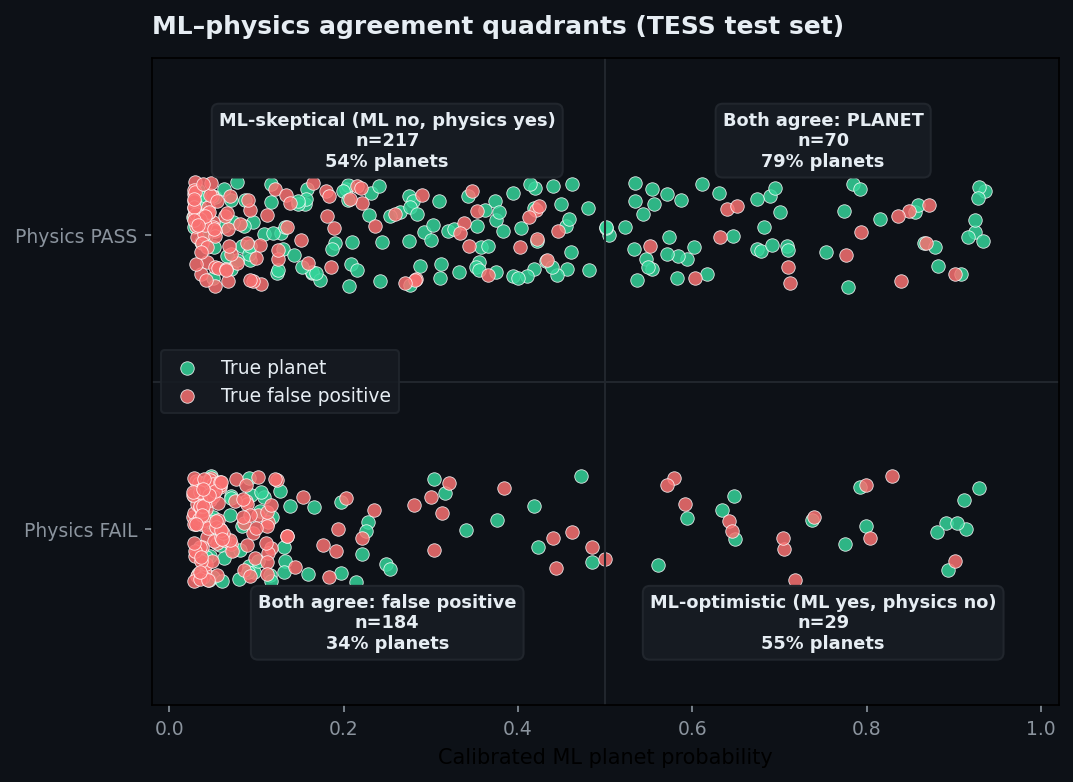
\includegraphics[width=0.62\linewidth]{disagreement_quadrants.png}
\caption{ML--physics agreement quadrants on the TESS test set; box annotations
give the count and true-planet purity per quadrant.}
\label{fig:quad}
\end{figure}

\paragraph{Operationalizing it: follow-up efficiency.}
If disagreement carries information, using it should spend follow-up time better.
Figure~\ref{fig:triage} plots true planets recovered against the fraction of
targets observed, for four rankings. A physics-informed order (physics-pass first,
then probability) dominates probability alone throughout the early- and
mid-budget regime: its gain-curve area is $0.62$ vs.\ $0.59$ (random $0.50$,
oracle $0.75$), and it recovers half of all planets after observing $33\%$ of
targets vs.\ $39\%$ for probability alone. The improvement is modest but
consistent, and largest exactly where budgets bite --- early. This is direct,
operational evidence that the independent physics verdict, and the disagreement it
encodes, is worth acting on.

\begin{figure}[t]
\centering

\includegraphics[width=0.62\linewidth]{triage_efficiency.png}
\caption{Follow-up efficiency: cumulative true planets recovered vs.\ fraction of
targets observed. Physics-informed rankings beat ML probability alone in the
budget-limited regime.}
\label{fig:triage}
\end{figure}

\section{Ablations}
Leave-one-group-out feature ablation (retraining on Kepler, testing on TESS) shows
the SNR and shape features carry most of the transferable signal; dropping depth
features slightly \emph{helps}, consistent with depth being the most
mission-specific feature. A physics-check ablation on the TESS false positives
shows the five checks together flag $57.5\%$ of them, with SDE and the odd/even
test contributing most --- orthogonal rejection the learned score does not supply.
Full tables are in \texttt{research/results/}.

\section{Validation}
Several checks confirm the results are real rather than pipeline artifacts
(Figure~\ref{fig:perm}). A permutation test --- shuffling the TESS labels
$5000\times$ --- collapses the AUC to a null centered at $0.50$ ($[0.41,0.59]$),
with the observed $0.68$ far outside it ($p=0$); the cross-mission signal is
genuine. The physics-pass/label association is strong (Fisher exact odds ratio
$4.1$, $p=5\times10^{-5}$), so the disagreement finding is not noise. For all
$107$ period-recovered targets the TLS period matches the independent ExoFOP
catalog period to within $3\%$ (median error $0.08\%$), confirming detections are
real, not spurious. Training (Kepler KIC/KOI) and test (TESS TIC) target sets are
disjoint by construction, precluding leakage. The one honest negative: the
\emph{thresholded} ML prediction alone is only weakly associated with truth on
TESS (Fisher $p=0.11$) --- precisely the transfer weakness the physics vetting
compensates for.

\begin{figure}[t]
\centering

\includegraphics[width=0.58\linewidth]{validation_permutation.png}
\caption{Permutation test: the observed cross-mission AUC lies far outside the
label-shuffled null distribution, so the signal is not a metric artifact.}
\label{fig:perm}
\end{figure}

\section{Discussion and limitations}
Our benchmark uses single-sector TESS light curves for tractability, which
lower-bounds detection performance; the three-sector experiment shows this helps
detection but not ranking. The $160$-target benchmark yields broad confidence
intervals; a larger sample would sharpen them. The 1D-CNN is trained on parametric
folded views rather than raw pixels; a full AstroNet-style detector is future work.
Injection hosts are screened for quietness but real correlated noise varies across
the sky. The benchmark is class-balanced ($50/50$) by construction, so the
quadrant purities are enrichments relative to a $50\%$ base rate; in the real,
planet-rare TOI population absolute purities would be lower while the \emph{relative}
ordering --- agreement pure, disagreement informative --- is what our claims rest
on. None of these change the central message: a detection pipeline is best
reported as a characterized decision system, and the disagreement between a
learned score and independent physics is a resource worth spending telescope time
on.

\section{Reproducibility}
Every figure and number regenerates from public archives:
\begin{center}\texttt{python -m research.run\_all}\end{center}
Code, the trained model, and result tables (with the exact values quoted here) are
in the repository; heavy stages are resumable.

\begin{thebibliography}{9}
\bibitem{shallue2018} Shallue, C.~J. \& Vanderburg, A. (2018). Identifying
Exoplanets with Deep Learning. \emph{AJ}, 155, 94.
\bibitem{exominer2021} Valizadegan, H.\ et al. (2022). ExoMiner. \emph{ApJ}, 926, 120.
\bibitem{exonet2026} ExoNet: Calibrated Multimodal Deep Learning for TESS
Exoplanet Candidate Vetting (2026), arXiv:2604.15560.
\bibitem{hippke2019tls} Hippke, M. \& Heller, R. (2019). Transit Least Squares.
\emph{A\&A}, 623, A39.
\end{thebibliography}

\end{document}
